\chapter{Introduction}

\section{Pourquoi chercher à reconstruire des sources de pollution?}
	La menace de rejets de substances \textit{Nucléaires}, \textit{Radiologiques}, \textit{Bactériologiques} ou \textit{Chimiques} (NRBC) dans l'atmosphère suscite un fort intérêt, du fait des enjeux humains et environnementaux qu'ils affectent. De tels incidents peuvent être d'origine accidentelle, causés par des rejets ayant eu lieu dans des sites industriels stockant ou exploitant des matières dangereuses. Plusieurs événements historiques témoignent de l'impact de tels accidents :\\
	\begin{itemize}
		\item Seveso (Italie) en 1976: un rejet accidentel de dioxine provenant d'une usine chimique engendre un nuage toxique contaminant une surface de près de 2.8 km$^2$, touchant plus de 400 personnes victimes de lésions cutanées, et nécessitant l'abattage de près de 80 000 bêtes contaminées dans les domaines agricoles atteints \cite{Seveso1976}. 
		
		\item Bhopal (Inde) en 1984: une explosion dans une usine de pesticides entraîne un important rejet de substances chimiques toxiques (isocyanathe de méthyle, cyanure hydrogéné) touchant directement la population vivant aux alentours. Le bilan a long terme est d'au moins 16 000 morts et environ 500 000 intoxiqués \cite{Bhopal1984}.
		
		\item Tchernobyl (Ukraine) en 1986: suite à des erreurs humaines lors d'opérations sur un réacteur de la centrale nucléaire locale, le c\oe{}ur est entré en fusion: il s'en est suivi une explosion et la libération d'importantes quantités d'éléments radioactifs dans l'atmosphère. Le nuage formé par ces polluants s'est répandu à l'échelle continentale sur une grande partie de l'Europe \cite{Repussard2006}.
		
		\item Algésiras (Espagne) en 1998: une usine espagnole incinère accidentellement une source radioactive dans ses hauts-fourneaux. Ce n'est que près de trois semaines plus tard que l'origine de la fuite est établie. Sur la base des mesures effectuées et de la reconstitution des courants atmosphériques, la quantité totale de césium 137 libérée a été évaluée à 1850 GBq \cite{Estevan2003}.
		
		\item Fukushima (Japon) en 2011: suite au déclenchement d'un séisme de magnitude 9.0 au large des côtes japonaises, les dégâts causés par le tsunami induit ont entraîné la fusion d'au moins deux réacteurs de la centrale de Fukushima, causant ainsi d'importants rejets radioactifs sur le territoire japonais, et plus largement, sur une large portion de l'océan Pacifique \cite{IRSN2012}.
		
		\item Igualada (Espagne) en 2015: une citerne explose en effectuant une livraison dans une usine chimique, causant la propagation d'un nuage orange d'acide nitrique. L'incident a entraîné des mesures de confinement des populations dans le voisinage immédiat de l'usine.
		\item Los Angeles (Etats-Unis) en 2015: une fuite localisée dans un puits de stockage de gaz de ville entraîne d'importants rejets de méthane dans l'atmosphère. L'incident a été déclaré le 23 octobre 2015, mais en janvier 2016 la brèche n'est toujours pas colmatée, et à cette date entre 30 et 50 tonnes par heure de méthane sont rejetés dans l'air. Le méthane étant un gaz à effet de serre, les conséquences environnementales à moyen et long terme sont déjà considérées comme graves.\\
	\end{itemize}
	
	Les incidents NRBC peuvent aussi être issus d'actes malveillants relevant du terrorisme. Ce fut le cas à Tokyo (Japon) en 1995, où des membres d'une secte ont percé des poches contenant du gaz sarin (un puissant neurotoxique) dans des rames de métro. Le bilan final fût  de 12 morts et plus de 5500 blessés. Plus récemment, le risque d'attentats NRBC a également été mis en évidence  en France suite aux attentats de l'année 2015, et amplifié en raison du contexte géopolitique actuel.\\
	
	Dans tous les cas, il est vital de disposer de techniques rapides pour détecter et évaluer le risque, afin d'assurer au mieux la sécurité des personnes et de coordonner les manoeuvres des équipes de premier secours. De telles techniques reposent sur des méthodes de modélisation des phénomènes physiques régissant l'atmosphère, ainsi que sur un système d'instrumentation permettant, entre autres, de caractériser et quantifier la présence de substances toxiques dans l'air.\\
	
	Cependant, pour que ces outils de modélisation puissent fonctionner, il est indispensable de disposer d'un certain nombre de paramètres, dont les caractéristiques de la source à l'origine du rejet. C'est ce point particulier que nous illustrerons dans la suite de ce chapitre, après un bref exposé introductif sur la physique de la dispersion atmosphérique.\\


	\section{Les principes de la dispersion atmosphérique}
	
	Nous décrivons ici les grandes lignes des règles physiques qui régissent la propagation d'un nuage de polluant dans l'atmosphère. Pour un exposé plus exhaustif, le lecteur peut se référer à \cite{Sportisse2008}.
	
	\subsection{L'équation d'advection-diffusion}
	
	Une fois qu'un polluant est émis dans l'atmosphère, son comportement est régi par plusieurs processus distincts:\\
	\begin{enumerate}
		\item le \textbf{transport}, ou \textbf{advection} qui se fait sous l'influence des circulations d'air dans l'atmosphère,
		\item la \textbf{diffusion}, résultant de la nature turbulente des écoulements dans la partie basse de l'atmosphère (couche limite),
		\item les processus de \textbf{pertes par dépôt sec ou humide}, diminuant la quantité de polluant transportée,
		\item les éventuelles \textbf{transformations physico-chimiques} pouvant altérer l'état du polluant lors de son séjour dans l'atmosphère: la filiation radioactive (s'il s'agit d'un radionucléide), ou les diverses réactions chimiques pouvant avoir lieu avec les autres composants de l'air.\\
	\end{enumerate}
	
	Nous supposerons en première approximation que les processus (3) et (4) énumérés précédemment ne sont pas pris en compte. Si on considère le transport d'un polluant unique dont la concentration peut être décrite au point $\bm{x} = (x,y,z) \in \mathbb{R}^3$ et à l'instant $t$ par une fonction $C(\bm{x},t)$. On peut alors écrire la loi de conservation de la masse pour $C$ sous la forme suivante:
	
	\begin{equation}
	\label{eqn_conservation_masse}
		\dfrac{\partial C}{\partial t} + \nabla \cdot \vec{J}(\bm{x},t) = \VecSigma
	\end{equation}
	où $\VecSigma$ est le \textit{terme source}, $\vec{J}(\bm{x},t)$ représente le flux de masse du polluant, et $\nabla$ désigne l'opérateur gradient. $\vec{J}$ est une fonction vectorielle qui regroupe la somme des phénomènes distincts d'advection et de diffusion: 
	\begin{equation}
	\label{eqn_somme_flux}
	\vec{J} = \vec{J}_A + \vec{J}_D
	\end{equation}
	Le terme $\vec{J}_D$ est associé au phénomène de diffusion. celui-ci est généralement considéré comme suivant la première loi de Fick, stipulant que le flux de diffusion $\vec{J}_D$ est proportionnel au gradient de concentration : 
	
	\begin{equation}
	\label{eqn_fick_diffusion}
	\vec{J}_D = - \bm{K}\nabla C
	\end{equation}
	où $\bm{K}$ est une matrice contenant les coefficients de diffusion moléculaire, qui dépendent de l'espèce du polluant. Le terme $\vec{J}_A$ est associé au phénomène d'advection, et traduit une dépendance linéaire de la concentration par rapport au champ de vent $\bm{\vec{u}}$:
	
	\begin{equation}
	\label{eqn_flux_advection}
	\vec{J}_A = C\bm{\vec{u}}
	\end{equation}
	La combinaison des équations \eqref{eqn_somme_flux}, \eqref{eqn_fick_diffusion} et \eqref{eqn_flux_advection} mène ainsi à la formulation de l'\textit{équation d'advection-diffusion}, formulée sur le modèle de \cite{Stockie2011}:\\
	
	\begin{equation}
		\label{eqn_advection_diffusion}
		\dfrac{\partial C}{\partial t} + \nabla \cdot(C\bm{\vec{u}}) = \nabla \cdot (\bm{K}\nabla C) + \VecSigma
	\end{equation}
	Cette équation constitue la base de départ pour les différents modèles numériques cherchant à simuler les phénomènes de dispersion atmosphérique.\\
	
	\subsection{Les différents modèles de dispersion}
	
	Suivant les situations, la taille du domaine sur lequel les calculs sont effectués peut grandement différer. On distingue habituellement : \\
	\begin{itemize}
		\item l'\textit{échelle locale}, aussi appelée \textit{micro-échelle} (jusqu'à 1 km): à ce niveau, des phénomènes spécifiques tels que la présence de bâtiments doivent être pris en compte dans le calcul des champs de vent.C'est à cette échelle qu'il convient de se placer pour traiter les études d'impact en milieu urbain (par exemple à l'échelle d'un quartier), ou sur un site industriel. 
		\item la \textit{méso-échelle}, ou \textit{échelle régionale} (jusqu'à 1000 km): elle est utilisée pour travailler sur des phénomènes plus larges, par exemple pour étudier l'impact de la pollution à l'ozone ou aux particules fines sur le territoire d'un pays tel que la France. 
		\item l'\textit{échelle planétaire}, ou \textit{échelle synoptique} ($>$ 1000 km): on s'intéresse ici à l'impact d'événements de très grande ampleur, tels que les incidents de Tchernobyl ou Fukushima. \\
		
	\end{itemize}
	
	On peut également noter une certaine corrélation entre les échelles spatiales et temporelles dans le cadre accidentel: au niveau local, on s'intéresse typiquement à des phénomènes n'excédant pas quelques heures, alors qu'à l'échelle du globe on se place sur un intervalle de plusieurs semaines, voire plusieurs mois.\\ 
	
	Pour couvrir efficacement ces différentes tailles de zones, plusieurs types de modèles de dispersion existent. Ceux-ci se divisent en quatre catégories principales:\\
	
	\begin{itemize} 
		
	\item \textbf{Les modèles gaussiens}:
	Sous certaines hypothèses simplificatrices, l'équation \eqref{eqn_advection_diffusion} peut donner des solutions analytiques pour déterminer la concentration de polluant au sein de \textit{panaches} ou de \textit{bouffées} selon la configuration choisie. \cite{Stockie2011} résume les principes régissant les modèles gaussiens, et une présentation plus détaillée de leur fonctionnement sera introduite au Chapitre 3 du présent manuscrit.\\
	
	\item \textbf{Les modèles eulériens}:
	Le domaine de simulation sur lequel est résolue l'équation \eqref{eqn_advection_diffusion} est discrétisé en un maillage de calcul  par des méthodes numériques. On retrouve ce type d'approche dans des études de cas à l'échelle continentale \cite{Saunier2013} ou globale. \\
	
	\item \textbf{Les modèles lagrangiens particulaires}:
	Dans le cadre lagrangien, le rejet est modélisé comme un ensemble de particules numériques porteuses d'une masse élémentaire. Le modèle suit la trajectoire de chaque particule, dont le mouvement moyen est constitué d'une composante régie par le champ de vent, et d'une composante stochastique traduisant la variabilité causée par la turbulence. La concentration mesurée sur un volume élémentaire du domaine à un temps donné est ainsi égale à la somme des masses élémentaires portées par chaque particule contenue dans ce volume à cet instant. Ce type de modèle est présenté plus en détails au Chapitre 4.\\
	
	\item \textbf{Les modèles de mécanique des fluides}:
	Aussi appelés \textit{Computational Fluid Dynamics} (CFD), ces modèles sont utilisés à petite échelle, et impliquent une résolution des équations de Navier-Stokes sur un maillage relativement fin. Il en résulte une bonne précision des calculs, en particulier en cas de présence d'obstacles menant à des écoulements complexes.\\
	
	\end{itemize}
	
	
	\section{Les caractéristiques du terme source}
	
	Les modèles de dispersion présentés dans le paragraphe précédent nécessitent plusieurs types de données d'entrée: 
	\begin{itemize}
		\item un certain nombre de \textbf{paramètres météorologiques}: dans les cas simples, on peut utiliser la direction et la vitesse du vent (pouvant être choisis comme uniformes), ainsi que la classe de stabilité atmosphérique considérée. Dans des cas plus complexes, le modèle prend en entrée les mesures issues d'une station météo située dans le domaine d'étude ou à défaut, de la station la plus proche. Il peut également exploiter les résultats d'un système de prévision météo. Les grandeurs considérées sont alors la vitesse et la direction du vent, la température, l'humidité, la nébulosité et les flux de rayonnement.
		\item les \textbf{paramètres de la source} à l'origine des émissions à modéliser.
	\end{itemize}
	
	C'est sur ce second point que nous allons plus particulièrement nous pencher dans la suite de ce paragraphe.
	
	\subsection{Les différents types de source}
	
	La terminologie employée pour décrire la source d'un rejet polluant peut parfois prêter à confusion, car il existe plusieurs façons d'en décrire les caractéristiques. Nous fixons ici les termes utilisés pour distinguer les différents types de source rencontrés.\\
	
	Une source est dite \textit{localisée} si sa position peut être réduite à un point de l'espace, on peut également parler de \textit{source ponctuelle}. Par opposition, une \textit{source étendue} est caractérisée par une surface d'émission, il peut, par exemple, s'agir d'un bac de décantation dans une usine de retraitement des déchets, si on se place à une échelle suffisamment petite.\\
	
	Une source est également définie par le profil temporel de son rejet, autrement dit la variation de la quantité de polluant rejetée par unité de temps. Comme nous travaillons dans un cadre de modélisation numérique d'un phénomène physique, il est nécessaire de définir une discrétisation temporelle sur $T_s$ instants d'émission, sous la forme d'un vecteur $\bm{t'}_s = (t'_1, \dots, t'_{T_s})$. On peut alors construire le vecteur du profil d'émission comme étant la liste des quantités rejetées par pas de temps d'émission (figure \ref{fig_courbe_profil_source}) : 
	
	$$ \VecQSource = \left(q(t'_1), q(t'_2), \dots, q(t'_{T_s})\right)$$
	
	Si le rejet est suffisamment bref pour n'être effectif que sur un unique pas de temps, alors $\VecTSource$ est réduit à un scalaire $t'_s$, et $\VecQSource$ à une masse totale émise $q_s$ : dans ce cas, on parle d'une source dite \textit{instantanée}. Dans le cas inverse, et lorsque le débit n'est pas constant, on parle d'une source \textit{non-instantanée}. Si $ \forall i \in \{1, \dots, T_s\}, ~ q(t'_i)$ est constant, la source est dite \textit{continue}. \\
	
	
	\begin{figure}[hb]
		\centering
		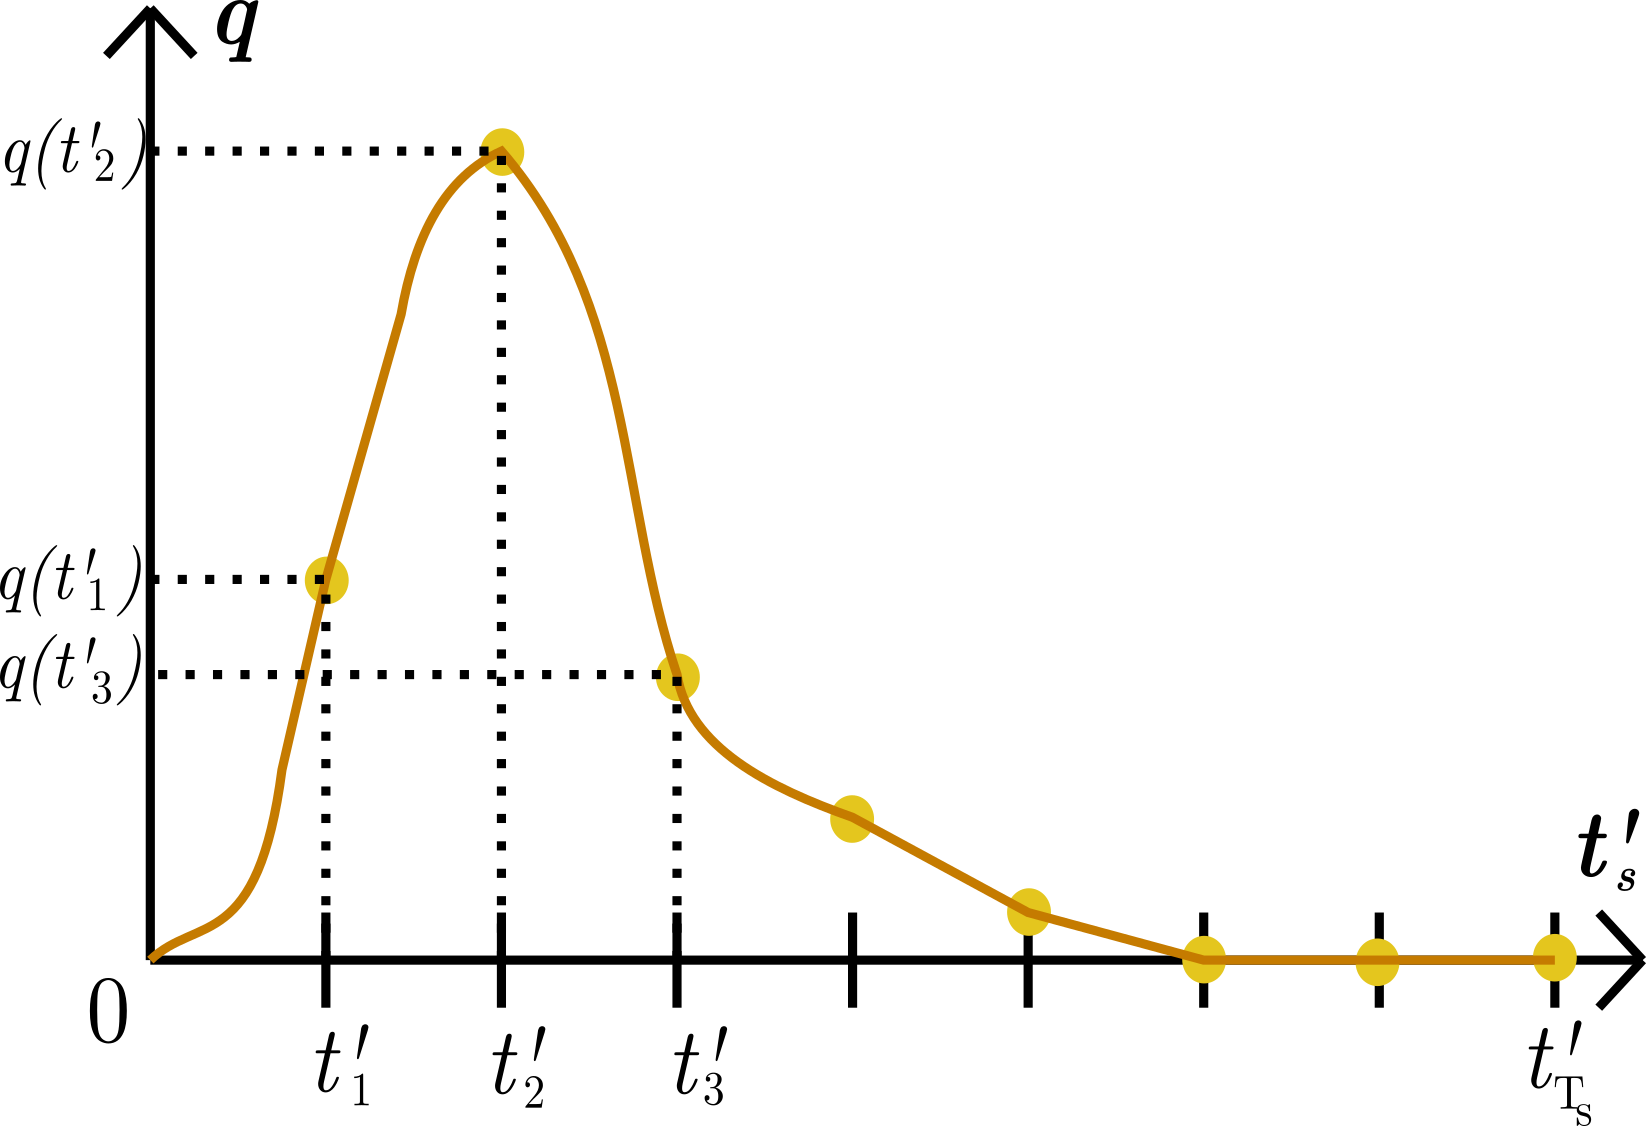
\includegraphics[scale=0.6]{courbe_profil_source.png}
		\caption{Exemple de discrétisation d'une source non-instantanée.}
		\label{fig_courbe_profil_source}
	\end{figure}
	
	Enfin, un cas d'étude peut comporter une \textit{source unique}, ou bien avoir une configuration \textit{multi-sources}.\\
%	
%	\subsection{Paramétrisation et relation source-récepteur}
%	
%	La façon la plus générale de formuler mathématiquement les caractéristiques d'un terme source consiste à définir un champ complet d'émission sur 4 dimensions (espace et temps), chaque élément de ce champ représentant une émission à un point et à un instant donnés. Si l'espace du domaine considéré est discrétisé en $N_xN_yN_z$ points, chaque point étant associé à un profil d'émission de longueur $T_s$, alors le terme source est défini comme un vecteur $\VecSigma \in \mathbb{R}^{N_\VecSigma}$ (où $N_\VecSigma = N_xN_yN_zT_s$).Il est ainsi possible de lier les observations générées par le modèle et le vecteur source $\VecSigma$ par la formule suivante, appelée \textit{relation source-récepteur}:
%	
%	
%	\begin{equation}
%		\label{eq_relation_SR_non_parametrique}
%		\VecObs = \bm{H}\VecSigma + \bm{\varepsilon}
%	\end{equation}
%	
%	où $\VecObs \in \mathbb{R}^m$ représente le vecteur des observations, $\VecSigma \in \mathbb{R}^{N_\VecSigma}$ la source discrétisée et $\bm{H} \in \mathbb{R}^{m \times N_\VecSigma}$  la \textit{matrice de transfert}. Le rôle de $\bm{H}$ est d'assurer la projection depuis l'espace $\mathbb{R}^{N_\VecSigma}$  de la source vers l'espace $\mathbb{R}^m$ des observations grâce à l'utilisation d'un modèle de dispersion atmosphérique. $\bm{\varepsilon} \in \mathbb{R}^m$ est le vecteur des erreurs d'observation, et prend en compte les erreurs de mesure, de représentativité et de modèle. \\
%	
%	Dans le cas particulier d'une source ponctuelle on peut, dans l'équation \eqref{eq_relation_SR_non_parametrique}, substituer $\VecSigma$ par un profil d'émission $\VecSigma$ issu d'un unique point du domaine spatial considéré. En procédant ainsi, il n'est plus nécessaire de définir arbitrairement un maillage conditionné par $N_x, N_y, N_z$  sur le domaine. De plus, la dimension du problème se réduit à estimer un point de l'espace et son profil temporel associé, soit $T_s + 3$ inconnues, contrairement au cas général où il faut retrouver l'intégralité du champ d'émission, soit $N_xN_yN_zT_s$ inconnues.\\
%	
%		
%	\section{Estimation du terme source: un état de l'art}
%	\label{section_etat_art_STE}
%	
%	\subsection{Une brève introduction aux problèmes inverses}
%	Le domaine des problèmes inverses constitue un vaste champ de la littérature scientifique, et de nombreux travaux y ont été menés. En pratique, résoudre un problème inverse revient à reconstituer un signal, une image, ou plus généralement une donnée non-observable à partir de mesures existantes, appelées observations.
%	Cette approche est duale à celle du problème direct où, à partir d'un signal ou d'un ensemble de paramètres initiaux, on cherche à en calculer les effets après une transformation donnée (figure \ref{fig_diagramme_direct_inverse}).
%	De nombreux domaines théoriques et pratiques font appel aux méthodes inverses. Le lecteur pourra trouver une revue complète de ces applications dans \cite{Tarantola2004}, on peut en citer quelques exemples tels que la géophysique \cite{Backus1967}, l'acoustique \cite{Kirsch1988}, l'imagerie satellite \cite{Park2003} et médicale \cite{Arridge1999}, les transferts thermiques \cite{McCormik1992} ou encore la finance quantitative \cite{Dembo1999}.\\
%	
%	\begin{figure}
%		\centering
%		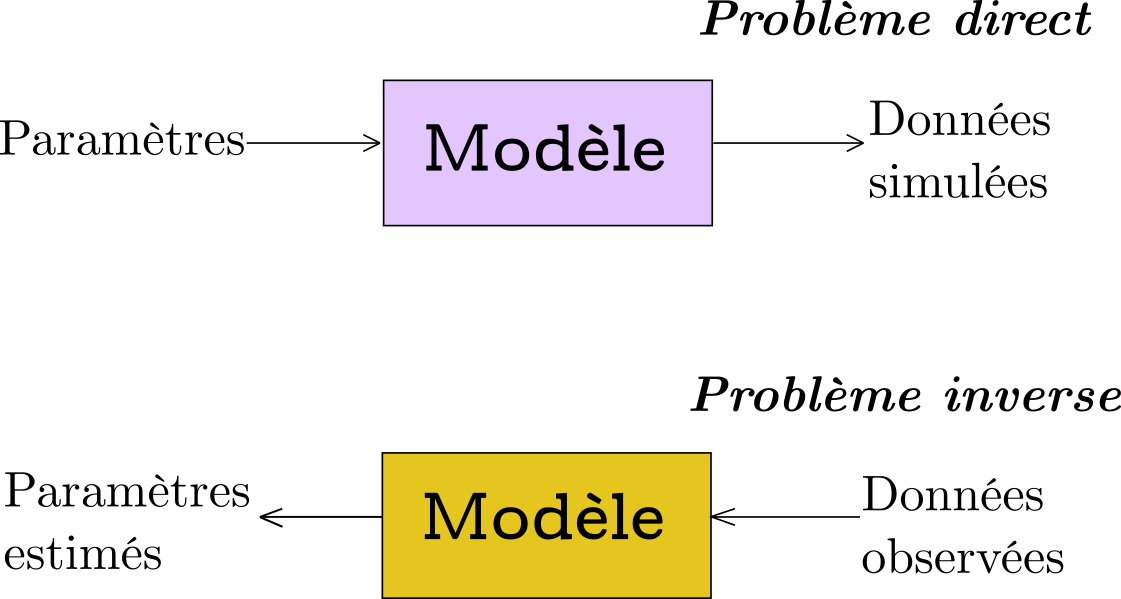
\includegraphics[scale=0.5]{diagramme_direct_inverse.png}
%		\caption{Schéma de principe illustrant la dualité entre problèmes direct et inverse.}
%		\label{fig_diagramme_direct_inverse}
%	\end{figure}
%	
%	
%	En dispersion atmosphérique, le problème direct peut ainsi se traduire par la donnée des paramètres de la source au modèle de dispersion, qui va produire le champ de concentration résultant. Cela revient bien à définir le problème inverse comme étant la reconstruction des paramètres de la source à partir des mesures de concentrations aux capteurs. Nous décrivons dans les paragraphes suivants les différentes approches existantes dans la littérature permettant de résoudre ce problème. Des éléments complémentaires sur la question sont également disponibles dans \cite{Rao2007}. Dans un souci de brièveté, par la suite nous qualifierons de "problèmes STE"(\textit{source term estimation) toutes les études de cas visant à estimer les paramètres d'une ou de plusieurs sources inconnues}.\\
%	
%	
% \subsection{Backtracking et modèles adjoints}
% 
% Une première possibilité consiste à étudier le problème dual associé à l'équation d'advection-diffusion  \eqref{eqn_advection_diffusion}, en inversant la flèche du temps, et par conséquent la direction du vent.  Par le principe de symétrie présenté dans \cite{Hourdin2006a}, on peut alors introduire la notion de \textit{rétro-transport} ou \textit{backtracking} en  réécrivant l'équation d'advection-diffusion sous la forme : 
% 
% \begin{equation}
% \label{eqn_advection_diffusion_backward}
% \dfrac{-\partial C^*}{\partial t} - \nabla \cdot(C^*\bm{\vec{u}}) = \nabla \cdot (\bm{K}\nabla C^*) + \VecObs
% \end{equation}
% 
% où $C^*$ est un champ de concentrations conjuguées, ou \textit{rétro-concentrations}, dont les valeurs sont obtenues par des rétro-rejets virtuels depuis les capteurs vers la source. Le modèle de dispersion associé à cette démarche duale est alors appelé \textit{modèle adjoint}, ou \textit{modèle backward}. Cette démarche revient ainsi à transformer le champ d'émission de \eqref{eq_relation_SR_non_parametrique} en un champ de rétro-émissions issues des capteurs, comme illustré sur les figures \ref{schema_probleme_direct} et \ref{schema_probleme_inverse}, et ainsi fournir une estimation qualitative du terme source.\\
% 
% \begin{figure}[h]
% 	\begin{subfigure}{0.5\textwidth}
% 		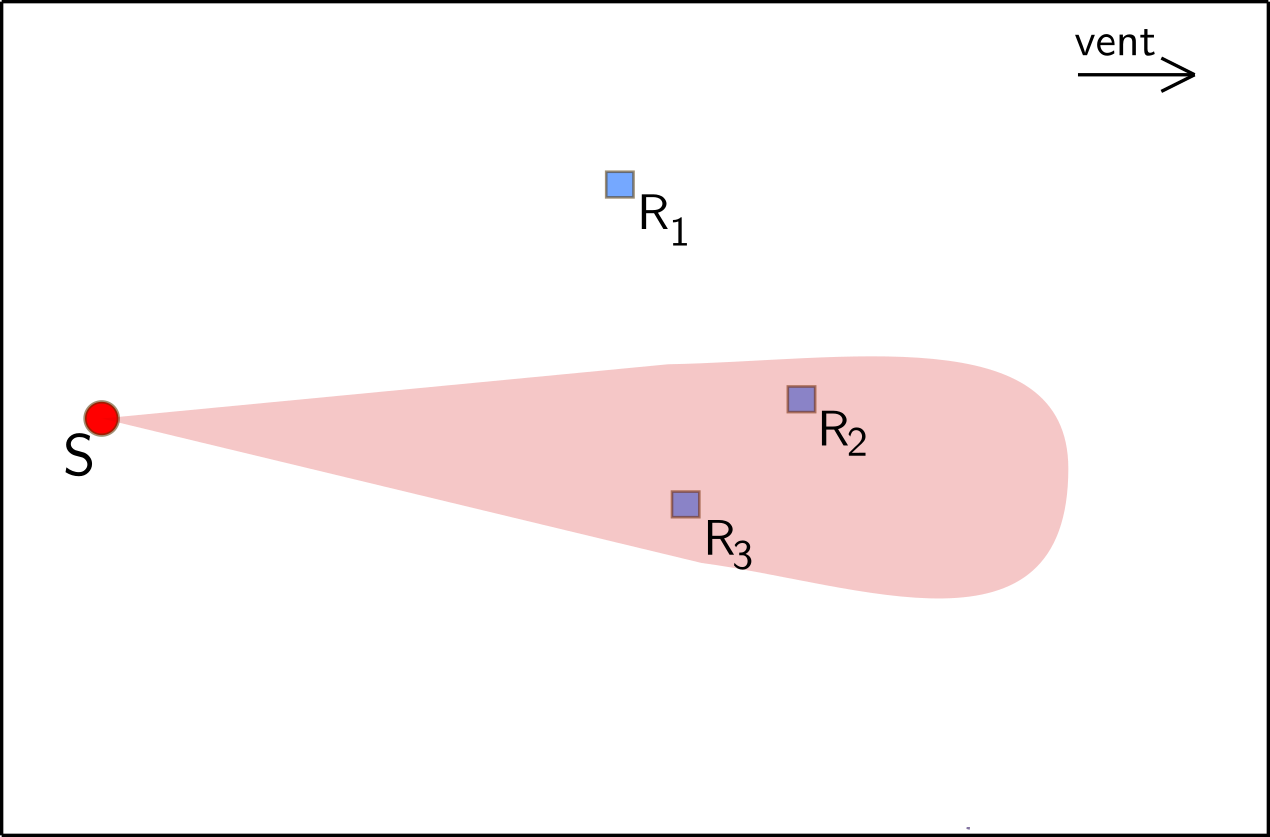
\includegraphics[scale=0.6]{schema_probleme_direct.png}
% 		\caption{Approche orientée source}
% 		\label{schema_probleme_direct}
% 	\end{subfigure}
% 	\begin{subfigure}{0.5\textwidth}
% 		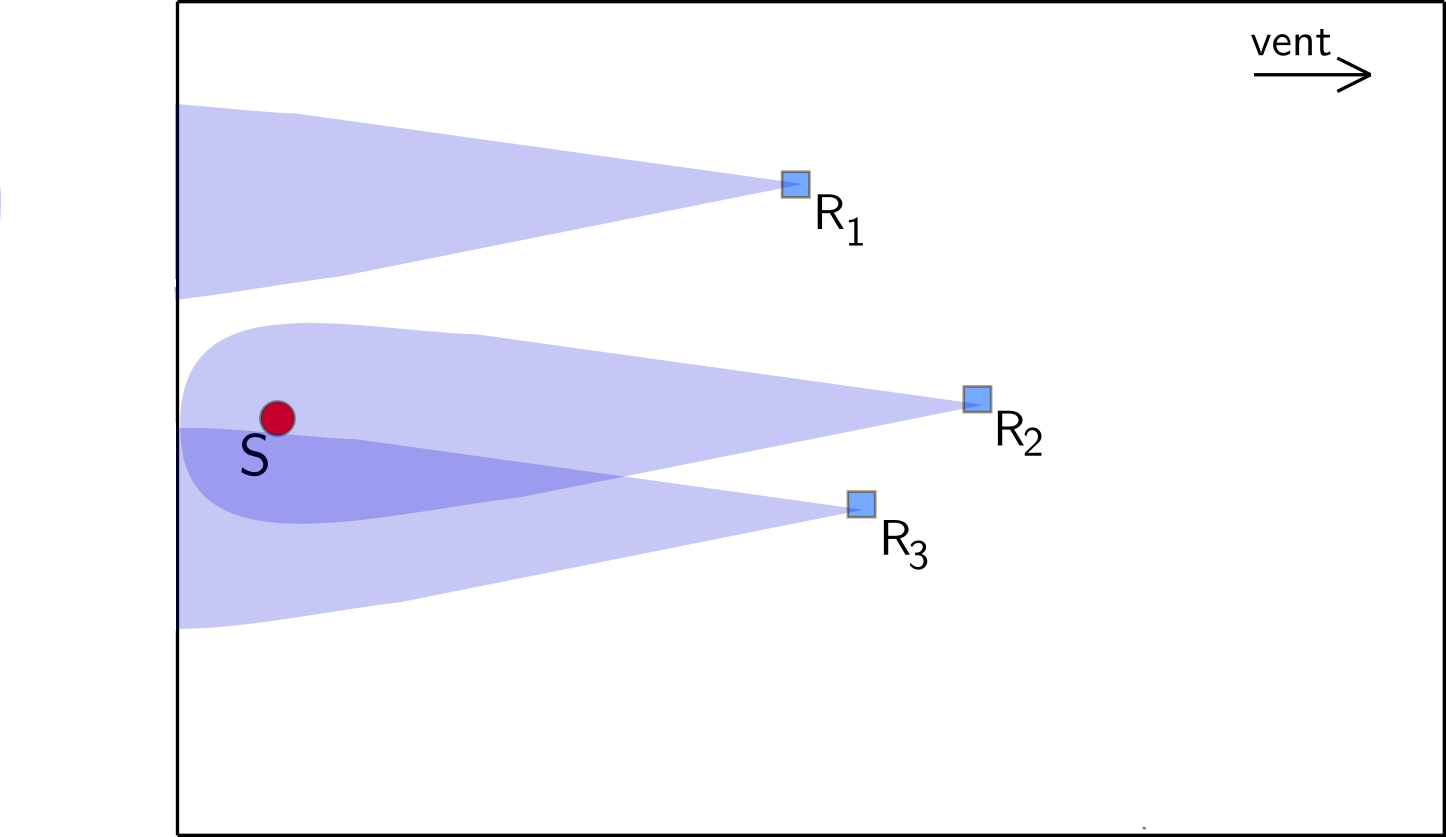
\includegraphics[scale=0.2]{schema_probleme_inverse.png}
% 		\caption{Approche orientée récepteur}
% 		\label{schema_probleme_inverse}
% 	\end{subfigure}
% 	\caption{Exemple illustrant la relation entre une source unique $S$ et trois capteurs $R_1,R_2,R_3$ sur un problème en deux dimensions pour les approches en "direct" (\ref{schema_probleme_direct}) et en "adjoint" (\ref{schema_probleme_inverse}). }
% \end{figure}
% 
% Dans \cite{Flesch1995}, un modèle \textit{backward} lagrangien est construit pour estimer le profil de rejet d'une source surfacique.  Cette méthode est également appliquée dans \cite{Pudykiewicz1998}, où la position et l'intensité du terme source de Tchernobyl sont reconstruits. De même, dans \cite{Hourdin2006b} le principe du \textit{backtracking} est appliqué à un modèle eulérien pour retrouver la source de la campagne ETEX\footnote{L’expérience \textit{European Tracer EXperiment} (ETEX), menée en 1997,  a consisté à mesurer et étudier l'impact à l'échelle européenne de rejets de gaz traceurs passifs émis depuis le nord de la France \cite{Nodop1998}.}.\\
% 
% \subsection{Optimisation et méthode des moindres carrés}
% \label{subsection_MCO}
% 
% L'équation \eqref{eq_relation_SR_non_parametrique} peut être réécrite sous la forme : 
% 
% \begin{equation}
% \VecObs = \widehat{\VecObs} + \VecErreur
% \label{eq_relation_SR_nonparam_simple}
% \end{equation}
%
%où $\widehat{\VecObs} = \MatH \VecSigma$ est l'approximation des observations $\VecObs$ par le processus de modélisation. On voit bien que dans le cas parfait où ce dernier reproduit exactement les observations attendues, on a $\VecErreur = 0$ et par suite $\widehat{\VecObs} = \VecObs$. Le fait de chercher la valeur $\VecSigma$ pour laquelle $\widehat{\VecObs}$ se rapproche le plus de $\VecObs$ permet ainsi de définir le problème STE sous la forme d'une minimisation de l'erreur $\VecErreur$: on définit pour cela une fonction-coût qui s'écrit : 
%
%\begin{equation}
%\CostF(\VecSigma) = ||\VecObs - \MatH \VecSigma||_p = ||\VecObs- \widehat{\VecObs}||_p
%\label{eq_cost_function_definition}
%\end{equation}
%où $||\cdot||_p$ désigne une norme $L_p$ arbitrairement choisie. La résolution du problème STE se traduit alors par la minimisation de cette fonction-coût:
%
%\begin{equation}
%\widehat{\VecSigma} = \argmin_\VecSigma \mathcal{J}(\VecSigma)
%\label{eq_argmin_cost_function}
%\end{equation}
%où $\widehat{\VecSigma}$ est l'estimation du terme source recherchée. Il existe différentes approches  pour aborder ce problème d'optimisation, qui est ici posé dans un cas générique. Dans ce paragraphe, nous étudions une des méthodes les plus courantes pour résoudre l'équation \eqref{eq_argmin_cost_function}, à savoir la méthode des \textit{moindres carrés ordinaires} (MCO). Celle-ci consiste à choisir une norme $L_2$ pour la définition de la fonction-coût, ainsi qu'un écart quadratique entre $\widehat{\VecObs}$ et $\VecObs$ : 
%
%\begin{equation}
%\CostF_{2}(\VecSigma) = ||\VecObs - \MatH \VecSigma ||_2^2
%\label{eq_cost_MCO}
%\end{equation}
%
%L'erreur que nous cherchons à minimiser est une combinaison des différentes sources d'erreur existantes (mesure, représentativité, modèle). Comme il est difficile de quantifier les contributions respectives de chacune de ces erreurs, on peut invoquer le principe du maximum d'entropie pour définir la représentation statistique de l'ensemble de ces erreurs comme étant un bruit gaussien centré et de matrice de covariance $\MatR$ : 
%
%\begin{equation}
%\VecErreur \sim \mathcal{N}(0,\MatR)
%\label{eq_bruit_obs}
%\end{equation}
%
%La fonction-coût peut alors s'écrire sous la forme suivante \cite{Winiarek2011}:
%
%\begin{equation}
%\mathcal{J}_2(\VecSigma) = \dfrac{1}{2}(\VecObs - \MatH \VecSigma)^T \MatR^{-1}(\VecObs - \MatH\VecSigma)
%\label{eq_cost_forme2}
%\end{equation}
%
%Sous cette hypothèse, minimiser $\CostF_2$ revient de façon équivalente à calculer l'estimateur du \textit{maximum de vraisemblance} (EMV), i.e. à maximiser la quantité $p(\VecObs | \VecSigma)$: 
%
%\begin{equation}
%\widehat{\VecSigma_2} = \argmax_\VecSigma~ p(\VecObs | \VecSigma)
%\label{eq_ML_MCO}
%\end{equation}
%
%Dans \cite{Kathirgamanathan2002}, un point source instantané est estimé à l'aide d'une méthode des moindres carrés, cette source étant caractérisée par sa masse totale émise, sa position et son instant d'émission. L'étude qui y est menée met notamment l'accent sur l'influence du dimensionnement du réseau de capteurs sur la performance de la reconstruction : au moins trois points de mesure sont nécessaires, et la distance entre les différents capteurs influe sur la qualité de l'estimation.\\
%
%Dans \cite{Ryall2001}, ce sont des zones d'émission plus grandes qui sont estimées pour des rejets de gaz à effet de serre sur plusieurs années. \\
%
%Dans \cite{Matthes2005}, une approche en deux temps est formulée afin de résoudre un problème de complexité proportionnellement croissante au nombre de capteurs. Dans une première étape, les mesures individuelles de chaque capteur produisent des ensembles de positions probables pour la source. Dans un deuxième temps, ces ensembles sont comparés pour estimer la meilleure position en faisant varier l'intensité de la source à retrouver. \\
%
% Dans \cite{Robertson1998}, l'inversion est faite dans le cadre de l'assimilation de données: cette méthodologie permet de corriger de façon variationnelle les paramètres du modèle de dispersion selon une boucle de rétro-action basée sur des observations. Très utilisée en météorologie, l'assimilation de données agit en deux temps selon un principe de "prévision-correction", et itère sur le cycle suivant:
% \begin{enumerate}
% 	\item  on calcule d'abord une ébauche de l'état à l'instant présent $t$, en appliquant un modèle de prévision en $t-1$,
% 	\item  on exploite ensuite les observations disponibles à l'instant $t$ pour corriger les paramètres du modèle en les comparant avec l'ébauche. \\
% \end{enumerate}
% 
% \cite{Issartel2005} mentionne le principe d'\textit{illumination}, qui est une mesure quantitative de la représentativité des mesures dans le temps et l'espace. Dans le cadre d'un modèle adjoint, l'illumination permet ainsi de caractériser des zones qui ne sont pas forcément couvertes par les rétro-émissions issues des capteurs, par exemple si la zone considérée est relativement éloignée du point de mesure le plus proche. Cependant, si l'information d'illumination est utilisée pour inverser un terme source, alors elle aura tendance à fortement favoriser les solutions proches des capteurs. Pour compenser ce problème, une phase de \textit{renormalisation} est introduite (\cite{Issartel2007} et \cite{Sharan2009}) pour équilibrer l'information apportée par chacun des capteurs. D'abord utilisée à grande échelle, cette méthodologie a récemment été validée à l'échelle locale dans \cite{Singh2014}, et dans un contexte urbain par \cite{Kumar2015}. \\
% 
% 
% \subsection{Algorithmes évolutionnaires}
% 
% Le problème d'optimisation posé par l'équation \eqref{eq_argmin_cost_function} peut également se résoudre par le biais de \textit{métaheuristiques} (méthodes d'optimisation généralement appliquées des problèmes à forte complexité combinatoire). Parmi celles-ci, les \textit{approches évolutionnaires}, et en particulier les \textit{algorithmes génétiques} ont été utilisés à plusieurs reprises pour résoudre des problèmes STE.\\
% 
%Les algorithmes évolutionnaires s'inspirent du principe de l'évolution darwinienne des populations biologiques, et leur construction s'appuie sur le fait que l'apparition d'espèces adaptées au milieu est la conséquence de la conjonction de deux phénomènes distincts : 
%
% \begin{itemize}
% 	\item d'une part, la \textit{sélection naturelle} imposée par le milieu (les individus les plus adaptés survivent et se reproduisent),
% 	\item d'autre part, les variations non-contrôlées du matériel génétique des espèces.
% \end{itemize}
% 
% Pour un problème d'optimisation standard, la fonction-coût $\CostF$ à minimiser devient, dans le langage évolutionnaire, une \textit{fonction d'adaptation}. Les points du domaine $\Omega$ des paramètres à explorer sont appelés \textit{individus}, et l'ensemble d'individus est appelé \textit{population}. \\
% 
% La structure d'un algorithme évolutionnaire se compose de plusieurs étapes. Dans un premier temps, on initialise une population $\Pi_0$ en tirant $p$ individus dans $\Omega$ de façon uniformément aléatoire, et on l'évalue en calculant les valeurs de $\CostF$ pour chaque individu. Vient ensuite une boucle itérative qui implémente le processus de sélection naturelle:
% \begin{enumerate}
% 	\item on sélectionne les individus les plus performants (au sens de $\CostF$) de la population $\Pi_i$ à l'itération courante $i$, que l'on appelle \textit{parents},
% 	\item on applique des opérateurs de variation aux parents sélectionnés, pour générer de nouveaux individus: les \textit{enfants}. On parle de mutation si l'opérateur est 1-aire (i.e. ne prend qu'un seul individu en argument) et de croisement si l'opérateur est $n$-aire (i.e. prend $n$ individus en argument, avec $n \geq 2$). Notons que cette étape est purement stochastique, et que les opérateurs n'utilisent pas d'information sur la performance des précédentes générations: on parle alors d'opérateurs semi-aveugles.
% 	\item on évalue les enfants avec $\CostF$,
% 	\item on remplace $\Pi_i$  par une nouvelle population $\Pi_{i+1}$ créée à partir des enfants et des parents de $\Pi_i$ au moyen d'une sélection darwinienne.\\
% \end{enumerate}
% 
% Dans notre contexte, on peut assimiler $\Omega$ à l'espace des paramètres du terme source. Historiquement, les premières méthodes d'estimation basées sur les algorithmes génétiques (voir par exemple \cite{Haupt2005}) supposaient connues certaines informations a priori comme les emplacements potentiels de la source. Dans \cite{Allen2007} et \cite{Haupt2007}, il est envisagé de se placer dans une situation plus réaliste où les paramètres à estimer comprennent non seulement la position de la source et la masse totale émise, mais également la vitesse et la direction du vent. \cite{Cervone2011} propose une extension du processus de variation en couplant les opérateurs de croisement et de mutation avec un algorithme non-darwinien d'inférence statistique.\\ 
% 
% Une telle approche a également permis d'étudier le rapport entre la précision du terme source reconstruit et le nombre de capteurs utilisés. \cite{Long2010} reprend ce problème de précision en testant un algorithme génétique sur différentes configurations de réseaux de capteurs plus ou moins denses, et en prenant en compte le caractère bruité des données fournies par les détecteurs. \\
% 
% L'approche génétique a récemment été validée sur des données expérimentales de rejet multi-sources, comme présenté dans les travaux de \cite{Cantelli2015} où jusqu'à trois sources distinctes ont pu être caractérisées.\\
% 
% \subsection{Méthodes bayésiennes déterministes}
% 
% Plusieurs travaux de la littérature STE privilégient une approche \textit{bayésienne}\footnote{Nous décrirons plus en détail les principes fondamentaux de la statistique bayésienne dans le prochain chapitre.} à celle du maximum de vraisemblance présentée au paragraphe §\ref{subsection_MCO}. Concrètement, ces travaux considèrent la distribution a posteriori $p(\VecSigma|\VecObs)$ du terme source comme étant la grandeur d'intérêt, celle-ci pouvant s'exprimer en fonction de la vraisemblance $p(\VecObs | \VecSigma)$ et de l'information a priori $p(\VecSigma)$ disponible sur $\VecSigma$ grâce à la règle de Bayes : 
% 
% \begin{equation}
% p(\VecSigma|\VecObs) = \dfrac{p(\VecObs | \VecSigma)p(\VecSigma)}{p(\VecObs)}
% \label{eq_regle_bayes_edl}
% \end{equation}
% 
%Le fait d'utiliser un a priori sur $\VecSigma$ dans le cadre bayésien revient, dans un cadre d'optimisation, à introduire une \textit{ébauche} du terme source, parfois appelée \textit{first-guess} ou \textit{background}, que nous noterons $\VecSigmaB$
%
%\subsubsection{Régularisation $L_2$}
%
%On met ici l'équation \eqref{eq_cost_MCO} sous la forme: 
% 
% \begin{equation}
% \mathcal{J}_{2_B}(\VecSigma) = ||\VecObs - \MatH \VecSigma||_2^2 + \lambda_B ||\VecSigmaB||_2
% \label{eq_cost_MCO_reg}
% \end{equation}
% 
% L'équation \eqref{eq_cost_MCO_reg} illustre le principe de la régularisation de Tikhonov \cite{Tikhonov1963}, qui permet de traiter des problèmes inverses mal-posés\footnote{Un problème bien-posé au sens de Hadamard \cite{Hadamard1902} désigne un modèle mathématique dont la solution existe, est unique, et dépend de façon continue des données. A l'inverse, un problème mal-posé déroge à au moins une des règles précédemment citées. De nombreux problèmes physiques sont mal-posés et nécessitent d'être \textit{régularisés} afin de pouvoir être traités.} du fait du faible nombre d'observations et de la faible observabilité potentielle de la source, qui engendrent une infinité de solutions. L'ajout du terme régularisant $\lambda_B ||\VecSigmaB||_2$ permet ainsi de garantir l'unicité de la solution du problème inverse. \\
% 
% Dans le cas des statistiques gaussiennes (équation \eqref{eq_bruit_obs}), l'erreur d'ébauche $\VecSigma - \VecSigmaB$ suit également une loi normale centrée, de matrice de covariance $\MatB$:
% 
% \begin{equation}
% (\VecSigma - \VecSigmaB) \sim \mathcal{N}(0,\MatB)
% \label{eq_erreur_ebauche}
% \end{equation}
% 
% L'équation \eqref{eq_cost_forme2} devient alors \cite{Winiarek2011}:
%
%\begin{equation}
%\mathcal{J}_2(\VecSigma) = \dfrac{1}{2}(\VecObs - \MatH \VecSigma)^T \MatR^{-1}(\VecObs - \MatH\VecSigma) + \dfrac{1}{2}(\VecSigma - \VecSigmaB)^T\MatB^{-1}(\VecSigma - \VecSigma)
%\label{eq_cost_reg_forme2}
%\end{equation}
%Le terme de droite fait ici office de régularisant. \\
%
%Dans \cite{Winiarek2012}, un estimateur ponctuel de type \textit{maximum a posteriori} (MAP) est utilisé pour résoudre un problème STE à l'échelle continentale, cet estimateur est obtenu en calculant le \textit{Best Linear Unbiased Estimator} (BLUE), qui est une méthode basée sur une descente de gradient. \\
%
%Dans le même cadre, \cite{Saunier2013} propose une reconstruction du terme source de l'accident de Fukushima en deux temps. Tout d'abord, une première fonction-coût est minimisée pour estimer la période du rejet, puis tenant compte de cette contrainte, une seconde fonction-coût est optimisée pour retrouver la source à proprement parler. 
%Il est à noter que l'équation \eqref{eq_cost_reg_forme2} correspond à celle de la méthode d'assimilation variationnelle de données 3D-var \cite{Courtier1998}. La vision de ce type d'estimation se rapproche ainsi de celle de l'assimilation de mesures issues de capteurs pour reconstruire un état inconnu, qui est ici le champ d'émission de la source recherchée.\\
%
%Une variante pour cette approche consiste à se placer dans un cadre statistique non-gaussien, notamment si on cherche à caractériser l'ébauche suivant certaines hypothèses spécifiques \cite{Bocquet2005a}. Les auteurs de \cite{Krysta2007} font l'hypothèse d'une source ponctuelle et instantanée pour définir une forme particulière d'ébauche, et utilisent un principe de maximum d'entropie sur la moyenne \cite{Jaynes1957} pour réécrire la fonction-coût et en dériver un estimateur approprié pour $\VecSigma$.\\
%
%\subsubsection{Régularisation $L_1$}
%
%Il peut exister des situations où les observations prennent l'allure de \textit{signaux parcimonieux}, autrement dit elles sont décrites par un très faible nombre de valeurs non-nulles sur l'intervalle temporel de mesure. C'est par exemple le cas dans \cite{Martinez2013} où une étude sur les profils de rejets de xénon sous forme d'impulsions (ou \textit{short bursts}) est menée. Afin de prendre cela en compte, l'équation \eqref{eq_cost_MCO} est modifiée et c'est cette fois un terme régularisant sous une norme $L_1$ qui est utilisé: 
%
%\begin{equation}
%\mathcal{J}_{2_L} = ||\VecObs - \MatH\VecSigma||_2^2 + \lambda_L ||\VecSigma||_1
%\label{eq_MCO_L1}
%\end{equation}
%
%Dans une optique bayésienne, cela revient à introduire une information a priori de parcimonie sous la forme d'une loi laplacienne sur $p(\VecSigma)$ et à calculer un estimateur de type LASSO \cite{Tibshirani1996}.
%
%
%\subsection{Méthodes de simulation stochastique}
%
%Afin d'avoir une solution au problème STE qui puisse être bien décrite du point de vue statistique, dans le cadre bayésien il est préférable d'estimer l'entière distribution a posteriori $p(\VecSigma | \VecObs)$ au lieu de se limiter à un estimateur ponctuel tel que le MAP décrit précédemment.\\
%
%
%On peut prendre comme premier exemple l'étude menée par \cite{Sohn2002}, qui se penche sur le cas particulier de l'estimation de source à l'intérieur d'un bâtiment. Pour cela, un calcul initial simule un nombre $N$ fixé de scénarios $S_1,\dots,S_N$ possibles à partir d'un échantillon de paramètres $\VecTheta_1, \dots, \VecTheta_N$ potentiels de la source. Chaque scénario $S_k$ représente un jeu de mesures simulées issues d'une source de paramètres $\VecTheta_k$. Une fois cette collection constituée, la loi a posteriori suivante est calculée via la règle de Bayes, pour chaque scénario $S_k$:
%
%\begin{equation}
%\label{eq_bayes_monte_carlo}
%p(S_k|\VecObs) = \dfrac{p(S_k)p(\VecObs | S_k)}{p(\VecObs)}
%\end{equation}
%
%Cette première approche, appelée \textit{Bayes Monte Carlo} (BMC), permet de caractériser un rejet mais peut également servir à placer de façon optimale les capteurs d'un réseau de mesure. \\
%
%Toutefois, l'expression analytique de cette loi a posteriori n'est généralement  pas accessible de façon directe, du fait de la forte non-linéarité des phénomènes pris en compte par le modèle de dispersion. Il est alors nécessaire d'introduire des méthodes numériques d'approximation pour évaluer  $p(\VecSigma | \VecObs)$. En général, il s'agit d'algorithmes de simulation aléatoire appartenant à la famille des méthodes de Monte-Carlo, et qui permettent une exploration optimale de l'espace des solutions.\\
%
%Parmi ces algorithmes, la catégorie la plus connue est certainement celle des méthodes dites \textit{Markov Chain Monte-Carlo} (MCMC). Dans \cite{Keats2007} et \cite{Chow2008}, la méthode MCMC est employée dans un contexte urbain, et couplée à des modèles de dispersion suffisamment performants pour une prise en compte du milieu bâti. \cite{Senocak2008} propose l'utilisation d'un modèle de dispersion plus simple de type gaussien, amélioré par l'ajout de paramètres stochastiques relatifs à la diffusion turbulente, eux-mêmes estimés par l'algorithme MCMC en plus des paramètres de la source. , ce qui permet une exploitation plus efficace des calculs de dispersion. \cite{Yee2008b} étend la méthodologie aux cas où le nombre de sources est inconnu et considéré comme un paramètre supplémentaire à estimer, ajoutant ainsi une étape de sélection de modèle dans la procédure d'estimation. Cela est possible grâce à une méthode MCMC à \textit{sauts réversibles}, qui associe pour chaque nombre de sources possible un espace de paramètres différent à explorer. Enfin, \cite{Yee2014} propose une extension des concepts de \cite{Keats2007} à l'échelle globale, où un algorithme MCMC est utilisé pour reconstruire la position et le profil d'émission d'une usine d'isotopes médicaux à partir des mesures de xénon relevées par le réseau mondial des capteurs de l'OTICE\footnote{L'\textit{Organisation du Traité d'Interdiction Complète des Essais Nucléaires} (OTICE, ou CTBTO en anglais: \textit{Comprehensive Nuclear-Test Ban Treaty Organization)} a pour rôle de détecter, grâce à un réseau de capteurs déployés sur l'ensemble du globe, et de signaler à tous les pays signataires du traité toute explosion d'origine atomique, pour prendre des mesures afin d'empêcher les puissances nucléaires actuelles de poursuivre leurs essais, et les Etats ne disposant pas de l'arme atomique de s'en doter.}. \\

%\todo[inline]{Dans le cadre de ce manuscrit, la méthodologie MCMC est expliquée avec plus de détails au Chapitre 2 pour les aspects théoriques, et un exemple pratique d'application est illustré au Chapitre 3.\\}

\section{Problématique de recherche}

Le développement des méthodes STE dans le contexte de la dispersion atmosphérique est une branche scientifique relativement récente par rapport au cadre général de la physique de l'atmosphère. Il s'agit également d'un domaine de recherche largement pluridisciplinaire, mêlant des compétences en physique mais également sur des aspects mathématiques (optimisation, statistiques, simulation aléatoire...) et informatique (algorithmique, calcul scientifique haute performance...) variés. \\

Même si de nombreux aspects sont couverts par les éléments présents dans l'état de l'art exposé en paragraphe §\ref{section_etat_art_STE}, de nombreuses questions restent encore ouvertes. Dans le cas particulier de situations accidentelles, il est ainsi important pour les primo-intervenants de disposer d'une information fiable avec une certaine quantification de l'incertitude, à partir d'un nombre potentiellement faible de mesures, et dans un intervalle de temps raisonnablement court pour assurer l'efficacité de l'intervention. Les questions de vitesse de calcul sont alors, de fait, importantes: si elles ne posent pas de problèmes dans le cadre d'une étude \textit{a posteriori}, il en va autrement en situation de crise, où le temps de réponse à un incident est un paramètre primordial. Un autre aspect majeur est celui de la nature de la source à retrouver. Pour le contexte accidentel, si on se place dans le cas d'un attentat à la bombe sale ou dans celui d'une fuite sur un complexe industriel, l'hypothèse d'une source localisée est raisonnable. Toutefois il peut être intéressant de se pencher plus en détail sur le profil du rejet, celui-ci n'étant pas forcément instantané, alors que plusieurs méthodes privilégient l'estimation d'un unique instant d'émission $t'_s$. \\


\textit{Les travaux présentés dans ce manuscrit et ayant fait l'objet du travail de thèse ont donc pour but: }

\begin{itemize}
	\item \textit{de développer et valider une méthode basée sur l'inférence bayésienne, capable de caractériser un point source par sa localisation et son profil de rejet à partir de mesures issues d'un réseau de capteurs, }
	\item \textit{de coupler cette méthode avec un modèle de dispersion atmosphérique développé par ARIA Technologies et le CEA au sein d'une chaîne de calcul pouvant, à terme, être utilisée en situation opérationnelle.} \\
\end{itemize}


Pour cela, nous avons recours à une approche de type Monte-Carlo différente des MCMC de par sa philosophie, et basée sur un principe d'échantillonnage d'importance adaptatif. De telles méthodes permettent en effet une convergence suffisamment rapide, et pallient certaines difficultés rencontrées par les MCMC. Nous associons cette méthode adaptative, utilisée pour localiser la source, à un calcul analytique du profil d'émission, permis par le choix d'une hypothèse de gaussianité sur le vecteur $\VecSigma$, et accompagné par l'implémentation d'une étape de contrainte visant à assurer la positivité de $\VecSigma$. Le schéma d'implémentation que nous avons conçu permet ainsi de produire une estimation des paramètres de position et d'émission d'une source unique via un schéma itératif de couplage avec un modèle de dispersion, la procédure d'estimation à proprement parler demeurant indépendante du modèle choisi. \\

Pour développer cette thèse, le présent manuscrit est organisé de la façon suivante. Après avoir présenté la problématique posée par le sujet et effectué un premier tour d'horizon de la thématique dans ce chapitre introductif, nous développons au Chapitre 2 les principes régissant l'inférence bayésienne, en nous concentrant plus particulièrement sur les applications des méthodes de Monte-Carlo en statistique bayésienne. Nous y détaillons notamment le cheminement théorique permettant la construction de l'algorithme AMIS, qui constitue un élément central des travaux de cette thèse. 
Dans le Chapitre 3, nous présentons l'application de cet algorithme adaptatif à la question de la reconstruction du terme source en dispersion atmosphérique. Pour cela, nous exploitons un cas d'application pratique issu d'une campagne de mesures expérimentales dont nous expliquerons les conditions de réalisation. Le Chapitre 4 détaille une variante de la méthodologie présentée au Chapitre 3, avec l'utilisation d'une approche orientée récepteur, et l'emploi d'un code de dispersion de type lagrangien dans des configurations simulées de rase campagne et de milieu urbain.
Enfin, le Chapitre 5 conclut ce manuscrit et discute de plusieurs perspectives pour de futurs axes de prolongement de ces travaux.\\